% ----------------------------------------------------------------------
%
%                          Tesis.tex
%
%----------------------------------------------------------------------
%
% Este fichero contiene el "documento maestro" del documento. Lo \'unico
% que hace es configurar el entorno LaTeX e incluir los ficheros .tex
% que contienen cada secci\'on.
%
%----------------------------------------------------------------------
%
% Los ficheros necesarios para este documento son:
%
%       TeXiS/* : ficheros de la plantilla TeXiS.
%       Cascaras/* : ficheros con las partes del documento que no
%          son cap\'itulos ni ap\'endices (portada, agradecimientos, etc.)
%       Capitulos/*.tex : cap\'itulos de la tesis
%       Apendices/*.tex: ap\'endices de la tesis
%       constantes.tex: constantes LaTeX
%       config.tex : configuraci\'on de la "compilaci\'on" del documento
%       guionado.tex : palabras con guiones
%
% Para la bibliograf\'ia, adem\'as, se necesitan:
%
%       *.bib : ficheros con la informaci\'on de las referencias
%
% ---------------------------------------------------------------------

\documentclass[11pt,a4paper,twoside]{book}

%
% Definimos  el   comando  \compilaCapitulo,  que   luego  se  utiliza
% (opcionalmente) en config.tex. Quedar\'ia  mejor si tambi\'en se definiera
% en  ese fichero,  pero por  el modo  en el  que funciona  eso  no es
% posible. Puedes consultar la documentaci\'on de ese fichero para tener
% m\'as  informaci\'on. Definimos tambi\'en  \compilaApendice, que  tiene el
% mismo  cometido, pero  que se  utiliza para  compilar  \'unicamente un
% ap\'endice.
%
%
% Si  queremos   compilar  solo   una  parte  del   documento  podemos
% especificar mediante  \includeonly{...} qu\'e ficheros  son los \'unicos
% que queremos  que se incluyan.  Esto  es \'util por  ejemplo para s\'olo
% compilar un cap\'itulo.
%
% El problema es que todos aquellos  ficheros que NO est\'en en la lista
% NO   se  incluir\'an...  y   eso  tambi\'en   afecta  a   ficheros  de
% la plantilla...
%
% Total,  que definimos  una constante  con los  ficheros  que siempre
% vamos a querer compilar  (aquellos relacionados con configuraci\'on) y
% luego definimos \compilaCapitulo.
\newcommand{\ficherosBasicosTeXiS}{%
TeXiS/TeXiS_pream,TeXiS/TeXiS_cab,TeXiS/TeXiS_bib,TeXiS/TeXiS_cover,%
TeXiS/TeXiS_part%
}
\newcommand{\ficherosBasicosTexto}{%
constantes,guionado,Cascaras/bibliografia,config%
}
\newcommand{\compilaCapitulo}[1]{%
\includeonly{\ficherosBasicosTeXiS,\ficherosBasicosTexto,Capitulos/#1}%
}

\newcommand{\compilaApendice}[1]{%
\includeonly{\ficherosBasicosTeXiS,\ficherosBasicosTexto,Apendices/#1}%
}

%- - - - - - - - - - - - - - - - - - - - - - - - - - - - - - - - - - -
%            Pre\'ambulo del documento. Configuraciones varias
%- - - - - - - - - - - - - - - - - - - - - - - - - - - - - - - - - - -

% Define  el  tipo  de  compilaci\'on que  estamos  haciendo.   Contiene
% definiciones  de  constantes que  cambian  el  comportamiento de  la
% compilaci\'on. Debe incluirse antes del paquete TeXiS/TeXiS.sty
%---------------------------------------------------------------------
%
%                          config.tex
%
%---------------------------------------------------------------------
%
% Contiene la  definici\'on de constantes  que determinan el modo  en el
% que se compilar\'a el documento.
%
%---------------------------------------------------------------------
%
% En concreto, podemos  indicar si queremos "modo release",  en el que
% no  aparecer\'an  los  comentarios  (creados  mediante  \com{Texto}  o
% \comp{Texto}) ni los "por  hacer" (creados mediante \todo{Texto}), y
% s\'i aparecer\'an los \'indices. El modo "debug" (o mejor dicho en modo no
% "release" muestra los \'indices  (construirlos lleva tiempo y son poco
% \'utiles  salvo  para   la  versi\'on  final),  pero  s\'i   el  resto  de
% anotaciones.
%
% Si se compila con LaTeX (no  con pdflatex) en modo Debug, tambi\'en se
% muestran en una esquina de cada p\'agina las entradas (en el \'indice de
% palabras) que referencian  a dicha p\'agina (consulta TeXiS_pream.tex,
% en la parte referente a show).
%
% El soporte para  el \'indice de palabras en  TeXiS es embrionario, por
% lo  que no  asumas que  esto funcionar\'a  correctamente.  Consulta la
% documentaci\'on al respecto en TeXiS_pream.tex.
%
%
% Tambi\'en  aqu\'i configuramos  si queremos  o  no que  se incluyan  los
% acr\'onimos  en el  documento final  en la  versi\'on release.  Para eso
% define (o no) la constante \acronimosEnRelease.
%
% Utilizando \compilaCapitulo{nombre}  podemos tambi\'en especificar qu\'e
% cap\'itulo(s) queremos que se compilen. Si no se pone nada, se compila
% el documento  completo.  Si se pone, por  ejemplo, 01Introduccion se
% compilar\'a \'unicamente el fichero Capitulos/01Introduccion.tex
%
% Para compilar varios  cap\'itulos, se separan sus nombres  con comas y
% no se ponen espacios de separaci\'on.
%
% En realidad  la macro \compilaCapitulo  est\'a definida en  el fichero
% principal tesis.tex.
%
%---------------------------------------------------------------------


% Comentar la l\'inea si no se compila en modo release.
% TeXiS har\'a el resto.
% ���Si cambias esto, haz un make clean antes de recompilar!!!
\def\release{1}


% Descomentar la linea si se quieren incluir los
% acr\'onimos en modo release (en modo debug
% no se incluir\'an nunca).
% ���Si cambias esto, haz un make clean antes de recompilar!!!
%\def\acronimosEnRelease{1}


% Descomentar la l\'inea para establecer el cap\'itulo que queremos
% compilar

% \compilaCapitulo{01Introduccion}
% \compilaCapitulo{02EstructuraYGeneracion}
% \compilaCapitulo{03Edicion}
% \compilaCapitulo{04Imagenes}
% \compilaCapitulo{05Bibliografia}
% \compilaCapitulo{06Makefile}

% \compilaApendice{01AsiSeHizo}

% Variable local para emacs, para  que encuentre el fichero maestro de
% compilaci\'on y funcionen mejor algunas teclas r\'apidas de AucTeX
%%%
%%% Local Variables:
%%% mode: latex
%%% TeX-master: "./Tesis.tex"
%%% End:


% Paquete de la plantilla
\usepackage{TeXiS/TeXiS}
\usepackage{color}

% Incluimos el fichero con comandos de constantes
%---------------------------------------------------------------------
%
%                          constantes.tex
%
%---------------------------------------------------------------------
%
% Fichero que  declara nuevos comandos LaTeX  sencillos realizados por
% comodidad en la escritura de determinadas palabras
%
%---------------------------------------------------------------------

%%%%%%%%%%%%%%%%%%%%%%%%%%%%%%%%%%%%%%%%%%%%%%%%%%%%%%%%%%%%%%%%%%%%%%
% Comando: 
%
%       \titulo
%
% Resultado: 
%
% Escribe el t�tulo del documento.
%%%%%%%%%%%%%%%%%%%%%%%%%%%%%%%%%%%%%%%%%%%%%%%%%%%%%%%%%%%%%%%%%%%%%%
\def\titulo{AdaptaMaterialEscolar}

%%%%%%%%%%%%%%%%%%%%%%%%%%%%%%%%%%%%%%%%%%%%%%%%%%%%%%%%%%%%%%%%%%%%%%
% Comando: 
%
%       \autor
%
% Resultado: 
%
% Escribe los autores del documento.
%%%%%%%%%%%%%%%%%%%%%%%%%%%%%%%%%%%%%%%%%%%%%%%%%%%%%%%%%%%%%%%%%%%%%%
\def\autor{Pablo Miranda Torres\\Natalia Rodr�guez-Peral Valiente\\Jorge Velasco Conde}


%%%%%%%%%%%%%%%%%%%%%%%%%%%%%%%%%%%%%%%%%%%%%%%%%%%%%%%%%%%%%%%%%%%%%%
% Comando: 
%
%       \directores
%
% Resultado: 
%
% Escribe los directores del trabajo de fin de grado.
%%%%%%%%%%%%%%%%%%%%%%%%%%%%%%%%%%%%%%%%%%%%%%%%%%%%%%%%%%%%%%%%%%%%%%
\def\directores{Virginia Francisco Gilmart�n\\Raquel Herv�s Ballesteros}

%%%%%%%%%%%%%%%%%%%%%%%%%%%%%%%%%%%%%%%%%%%%%%%%%%%%%%%%%%%%%%%%%%%%%%
% Comando: 
%
%       \autorYDirectores
%
% Resultado: 
%
% Escribe primero los autores del documento, y despu�s los directores.
%%%%%%%%%%%%%%%%%%%%%%%%%%%%%%%%%%%%%%%%%%%%%%%%%%%%%%%%%%%%%%%%%%%%%%
\def\autorYDirectores{Pablo Miranda Torres\\Natalia Rodr�guez-Peral Valiente\\Jorge Velasco Conde\\[1.0em]
	{\Large Directores}\\[0.2em]
	\directores
}

%%%%%%%%%%%%%%%%%%%%%%%%%%%%%%%%%%%%%%%%%%%%%%%%%%%%%%%%%%%%%%%%%%%%%%
% Comando: 
%
%       \kanban
%
% Resultado: 
%
% Escribe Kanban con letra cursiva.
%%%%%%%%%%%%%%%%%%%%%%%%%%%%%%%%%%%%%%%%%%%%%%%%%%%%%%%%%%%%%%%%%%%%%%
\def\kanban{\textit{Kanban}}

% Variable local para emacs, para  que encuentre el fichero maestro de
% compilaci\'on y funcionen mejor algunas teclas r\'apidas de AucTeX

%%%
%%% Local Variables:
%%% mode: latex
%%% TeX-master: "tesis.tex"
%%% End:


% Sacamos en el log de la compilaci\'on el copyright
\typeout{Copyright Marco Antonio and Pedro Pablo Gomez Martin}

%
% "Metadatos" para el PDF
%
\ifpdf\hypersetup{%
    pdftitle = {\titulo},
    pdfsubject = {Plantilla de Tesis},
    pdfkeywords = {Plantilla, LaTeX, tesis, trabajo de
      investigaci\'on, trabajo de Master},
    pdfauthor = {\textcopyright\ \autor},
    pdfcreator = {\LaTeX\ con el paquete \flqq hyperref\frqq},
    pdfproducer = {pdfeTeX-0.\the\pdftexversion\pdftexrevision},
    }
    \pdfinfo{/CreationDate (\today)}
\fi


%- - - - - - - - - - - - - - - - - - - - - - - - - - - - - - - - - - -
%                        Documento
%- - - - - - - - - - - - - - - - - - - - - - - - - - - - - - - - - - -
\begin{document}

% Incluimos el  fichero de definici\'on de guionado  de algunas palabras
% que LaTeX no ha dividido como deber\'ia
%----------------------------------------------------------------
%
%                          guionado.tex
%
%----------------------------------------------------------------
%
% Fichero con algunas divisiones de palabras que LaTeX no
% hace correctamente si no se le da alguna ayuda.
%
%----------------------------------------------------------------

\hyphenation{
% a
abs-trac-to
abs-trac-tos
abs-trac-ta
abs-trac-tas
ac-tua-do-res
a-gra-de-ci-mien-tos
ana-li-za-dor
an-te-rio-res
an-te-rior-men-te
apa-rien-cia
a-pro-pia-do
a-pro-pia-dos
a-pro-pia-da
a-pro-pia-das
a-pro-ve-cha-mien-to
a-que-llo
a-que-llos
a-que-lla
a-que-llas
a-sig-na-tu-ra
a-sig-na-tu-ras
a-so-cia-da
a-so-cia-das
a-so-cia-do
a-so-cia-dos
au-to-ma-ti-za-do
% b
batch
bi-blio-gra-f�a
bi-blio-gr�-fi-cas
bien
bo-rra-dor
boo-l-ean-expr
% c
ca-be-ce-ra
call-me-thod-ins-truc-tion
cas-te-lla-no
cir-cuns-tan-cia
cir-cuns-tan-cias
co-he-ren-te
co-he-ren-tes
co-he-ren-cia
co-li-bri
co-men-ta-rio
co-mer-cia-les
co-no-ci-mien-to
cons-cien-te
con-si-de-ra-ba
con-si-de-ra-mos
con-si-de-rar-se
cons-tan-te
cons-trucci�n
cons-tru-ye
cons-tru-ir-se
con-tro-le
co-rrec-ta-men-te
co-rres-pon-den
co-rres-pon-dien-te
co-rres-pon-dien-tes
co-ti-dia-na
co-ti-dia-no
crean
cris-ta-li-zan
cu-rri-cu-la
cu-rri-cu-lum
cu-rri-cu-lar
cu-rri-cu-la-res
% d
de-di-ca-do
de-di-ca-dos
de-di-ca-da
de-di-ca-das
de-rro-te-ro
de-rro-te-ros
de-sa-rro-llo
de-sa-rro-llos
de-sa-rro-lla-do
de-sa-rro-lla-dos
de-sa-rro-lla-da
de-sa-rro-lla-das
de-sa-rro-lla-dor
de-sa-rro-llar
des-cri-bi-re-mos
des-crip-ci�n
des-crip-cio-nes
des-cri-to
des-pu�s
de-ta-lla-do
de-ta-lla-dos
de-ta-lla-da
de-ta-lla-das
di-a-gra-ma
di-a-gra-mas
di-se-�os
dis-po-ner
dis-po-ni-bi-li-dad
do-cu-men-ta-da
do-cu-men-to
do-cu-men-tos
% e
edi-ta-do
e-du-ca-ti-vo
e-du-ca-ti-vos
e-du-ca-ti-va
e-du-ca-ti-vas
e-la-bo-ra-do
e-la-bo-ra-dos
e-la-bo-ra-da
e-la-bo-ra-das
es-co-llo
es-co-llos
es-tu-dia-do
es-tu-dia-dos
es-tu-dia-da
es-tu-dia-das
es-tu-dian-te
e-va-lua-cio-nes
e-va-lua-do-res
exis-ten-tes
exhaus-ti-va
ex-pe-rien-cia
ex-pe-rien-cias
% f
for-ma-li-za-do
% g
ge-ne-ra-ci�n
ge-ne-ra-dor
ge-ne-ra-do-res
ge-ne-ran
% h
he-rra-mien-ta
he-rra-mien-tas
% i
i-dio-ma
i-dio-mas
im-pres-cin-di-ble
im-pres-cin-di-bles
in-de-xa-do
in-de-xa-dos
in-de-xa-da
in-de-xa-das
in-di-vi-dual
in-fe-ren-cia
in-fe-ren-cias
in-for-ma-ti-ca
in-gre-dien-te
in-gre-dien-tes
in-me-dia-ta-men-te
ins-ta-la-do
ins-tan-cias
% j
% k
% l
len-gua-je
li-be-ra-to-rio
li-be-ra-to-rios
li-be-ra-to-ria
li-be-ra-to-rias
li-mi-ta-do
li-te-ra-rio
li-te-ra-rios
li-te-ra-ria
li-te-ra-rias
lo-tes
% m
ma-ne-ra
ma-nual
mas-que-ra-de
ma-yor
me-mo-ria
mi-nis-te-rio
mi-nis-te-rios
mo-de-lo
mo-de-los
mo-de-la-do
mo-du-la-ri-dad
mo-vi-mien-to
% n
na-tu-ral
ni-vel
nues-tro
% o
obs-tan-te
o-rien-ta-do
o-rien-ta-dos
o-rien-ta-da
o-rien-ta-das
% p
pa-ra-le-lo
pa-ra-le-la
par-ti-cu-lar
par-ti-cu-lar-men-te
pe-da-g�-gi-ca
pe-da-g�-gi-cas
pe-da-g�-gi-co
pe-da-g�-gi-cos
pe-rio-di-ci-dad
per-so-na-je
plan-te-a-mien-to
plan-te-a-mien-tos
po-si-ci�n
pre-fe-ren-cia
pre-fe-ren-cias
pres-cin-di-ble
pres-cin-di-bles
pri-me-ra
pro-ble-ma
pro-ble-mas
pr�-xi-mo
pu-bli-ca-cio-nes
pu-bli-ca-do
% q
% r
r�-pi-da
r�-pi-do
ra-zo-na-mien-to
ra-zo-na-mien-tos
re-a-li-zan-do
re-fe-ren-cia
re-fe-ren-cias
re-fe-ren-cia-da
re-fe-ren-cian
re-le-van-tes
re-pre-sen-ta-do
re-pre-sen-ta-dos
re-pre-sen-ta-da
re-pre-sen-ta-das
re-pre-sen-tar-lo
re-qui-si-to
re-qui-si-tos
res-pon-der
res-pon-sa-ble
% s
se-pa-ra-do
si-guien-do
si-guien-te
si-guien-tes
si-guie-ron
si-mi-lar
si-mi-la-res
si-tua-ci�n
% t
tem-pe-ra-ments
te-ner
trans-fe-ren-cia
trans-fe-ren-cias
% u
u-sua-rio
Unreal-Ed
% v
va-lor
va-lo-res
va-rian-te
ver-da-de-ro
ver-da-de-ros
ver-da-de-ra
ver-da-de-ras
ver-da-de-ra-men-te
ve-ri-fi-ca
% w
% x
% y
% z
}
% Variable local para emacs, para que encuentre el fichero
% maestro de compilaci�n
%%%
%%% Local Variables:
%%% mode: latex
%%% TeX-master: "./Tesis.tex"
%%% End:


% Marcamos  el inicio  del  documento para  la  numeraci\'on de  p\'aginas
% (usando n\'umeros romanos para esta primera fase).
\frontmatter

%---------------------------------------------------------------------
%
%                          configCover.tex
%
%---------------------------------------------------------------------
%
% cover.tex
% Copyright 2009 Marco Antonio Gomez-Martin, Pedro Pablo Gomez-Martin
%
% This file belongs to the TeXiS manual, a LaTeX template for writting
% Thesis and other documents. The complete last TeXiS package can
% be obtained from http://gaia.fdi.ucm.es/projects/texis/
%
% Although the TeXiS template itself is distributed under the 
% conditions of the LaTeX Project Public License
% (http://www.latex-project.org/lppl.txt), the manual content
% uses the CC-BY-SA license that stays that you are free:
%
%    - to share & to copy, distribute and transmit the work
%    - to remix and to adapt the work
%
% under the following conditions:
%
%    - Attribution: you must attribute the work in the manner
%      specified by the author or licensor (but not in any way that
%      suggests that they endorse you or your use of the work).
%    - Share Alike: if you alter, transform, or build upon this
%      work, you may distribute the resulting work only under the
%      same, similar or a compatible license.
%
% The complete license is available in
% http://creativecommons.org/licenses/by-sa/3.0/legalcode
%
%---------------------------------------------------------------------
%
% Fichero que contiene la configuraci�n de la portada y de la 
% primera hoja del documento.
%
%---------------------------------------------------------------------


% Pueden configurarse todos los elementos del contenido de la portada
% utilizando comandos.

%%%%%%%%%%%%%%%%%%%%%%%%%%%%%%%%%%%%%%%%%%%%%%%%%%%%%%%%%%%%%%%%%%%%%%
% T�tulo del documento:
% \tituloPortada{titulo}
% Nota:
% Si no se define se utiliza el del \titulo. Este comando permite
% cambiar el t�tulo de forma que se especifiquen d�nde se quieren
% los retornos de carro cuando se utilizan fuentes grandes.
%%%%%%%%%%%%%%%%%%%%%%%%%%%%%%%%%%%%%%%%%%%%%%%%%%%%%%%%%%%%%%%%%%%%%%
\tituloPortada{AdaptaMaterialEscolar: Herramienta para la adaptaci�n de asignaturas a necesidades educativas especiales.
}

%%%%%%%%%%%%%%%%%%%%%%%%%%%%%%%%%%%%%%%%%%%%%%%%%%%%%%%%%%%%%%%%%%%%%%
% Autor del documento:
% \autorPortada{Nombre}
% Se utiliza en la portada y en el valor por defecto del
% primer subt�tulo de la segunda portada.
%%%%%%%%%%%%%%%%%%%%%%%%%%%%%%%%%%%%%%%%%%%%%%%%%%%%%%%%%%%%%%%%%%%%%%
\autorPortada{Pablo Miranda Torres\\Natalia Rodr�guez-Peral Valiente\\Jorge Velasco Conde}

%%%%%%%%%%%%%%%%%%%%%%%%%%%%%%%%%%%%%%%%%%%%%%%%%%%%%%%%%%%%%%%%%%%%%%
% Fecha de publicaci�n:
% \fechaPublicacion{Fecha}
% Puede ser vac�o. Aparece en la �ltima l�nea de ambas portadas
%%%%%%%%%%%%%%%%%%%%%%%%%%%%%%%%%%%%%%%%%%%%%%%%%%%%%%%%%%%%%%%%%%%%%%
\fechaPublicacion{Junio 2020}

%%%%%%%%%%%%%%%%%%%%%%%%%%%%%%%%%%%%%%%%%%%%%%%%%%%%%%%%%%%%%%%%%%%%%%
% Imagen de la portada (y escala)
% \imagenPortada{Fichero}
% \escalaImagenPortada{Numero}
% Si no se especifica, se utiliza la imagen TODO.pdf
%%%%%%%%%%%%%%%%%%%%%%%%%%%%%%%%%%%%%%%%%%%%%%%%%%%%%%%%%%%%%%%%%%%%%%
\imagenPortada{Imagenes/Vectorial/escudoUCM}
\escalaImagenPortada{.2}

%%%%%%%%%%%%%%%%%%%%%%%%%%%%%%%%%%%%%%%%%%%%%%%%%%%%%%%%%%%%%%%%%%%%%%
% Tipo de documento.
% \tipoDocumento{Tipo}
% Para el texto justo debajo del escudo.
% Si no se indica, se utiliza "TESIS DOCTORAL".
%%%%%%%%%%%%%%%%%%%%%%%%%%%%%%%%%%%%%%%%%%%%%%%%%%%%%%%%%%%%%%%%%%%%%%
\tipoDocumento{Trabajo de Fin de Grado}

%%%%%%%%%%%%%%%%%%%%%%%%%%%%%%%%%%%%%%%%%%%%%%%%%%%%%%%%%%%%%%%%%%%%%%
% Instituci�n/departamento asociado al documento.
% \institucion{Nombre}
% Puede tener varias l�neas. Se utiliza en las dos portadas.
% Si no se indica aparecer� vac�o.
%%%%%%%%%%%%%%%%%%%%%%%%%%%%%%%%%%%%%%%%%%%%%%%%%%%%%%%%%%%%%%%%%%%%%%
\institucion{%
Departamento de Ingenier�a del Software e Inteligencia Artificial\\[0.2em]
Facultad de Inform�tica\\[0.2em]
Universidad Complutense de Madrid
}

%%%%%%%%%%%%%%%%%%%%%%%%%%%%%%%%%%%%%%%%%%%%%%%%%%%%%%%%%%%%%%%%%%%%%%
% Director del trabajo.
% \directorPortada{Nombre}
% Se utiliza para el valor por defecto del segundo subt�tulo, donde
% se indica qui�n es el director del trabajo.
% Si se fuerza un subt�tulo distinto, no hace falta definirlo.
%%%%%%%%%%%%%%%%%%%%%%%%%%%%%%%%%%%%%%%%%%%%%%%%%%%%%%%%%%%%%%%%%%%%%%
%\directorPortada{Walterio Malatesta}

%%%%%%%%%%%%%%%%%%%%%%%%%%%%%%%%%%%%%%%%%%%%%%%%%%%%%%%%%%%%%%%%%%%%%%
% Texto del primer subt�tulo de la segunda portada.
% \textoPrimerSubtituloPortada{Texto}
% Para configurar el primer "texto libre" de la segunda portada.
% Si no se especifica se indica "Memoria que presenta para optar al
% t�tulo de Doctor en Inform�tica" seguido del \autorPortada.
%%%%%%%%%%%%%%%%%%%%%%%%%%%%%%%%%%%%%%%%%%%%%%%%%%%%%%%%%%%%%%%%%%%%%%


%%%%%%%%%%%%%%%%%%%%%%%%%%%%%%%%%%%%%%%%%%%%%%%%%%%%%%%%%%%%%%%%%%%%%%
% Texto del segundo subt�tulo de la segunda portada.
% \textoSegundoSubtituloPortada{Texto}
% Para configurar el segundo "texto libre" de la segunda portada.
% Si no se especifica se indica "Dirigida por el Doctor" seguido
% del \directorPortada.
%%%%%%%%%%%%%%%%%%%%%%%%%%%%%%%%%%%%%%%%%%%%%%%%%%%%%%%%%%%%%%%%%%%%%%
%\textoSegundoSubtituloPortada{%
%\textit{Versi�n \texisVer}
%}

%%%%%%%%%%%%%%%%%%%%%%%%%%%%%%%%%%%%%%%%%%%%%%%%%%%%%%%%%%%%%%%%%%%%%%
% \explicacionDobleCara
% Si se utiliza, se aclara que el documento est� preparado para la
% impresi�n a doble cara.
%%%%%%%%%%%%%%%%%%%%%%%%%%%%%%%%%%%%%%%%%%%%%%%%%%%%%%%%%%%%%%%%%%%%%%
%\explicacionDobleCara

%%%%%%%%%%%%%%%%%%%%%%%%%%%%%%%%%%%%%%%%%%%%%%%%%%%%%%%%%%%%%%%%%%%%%%
% \isbn
% Si se utiliza, aparecer� el ISBN detr�s de la segunda portada.
%%%%%%%%%%%%%%%%%%%%%%%%%%%%%%%%%%%%%%%%%%%%%%%%%%%%%%%%%%%%%%%%%%%%%%
%\isbn{978-84-692-7109-4}


%%%%%%%%%%%%%%%%%%%%%%%%%%%%%%%%%%%%%%%%%%%%%%%%%%%%%%%%%%%%%%%%%%%%%%
% \copyrightInfo
% Si se utiliza, aparecer� informaci�n de los derechos de copyright
% detr�s de la segunda portada.
%%%%%%%%%%%%%%%%%%%%%%%%%%%%%%%%%%%%%%%%%%%%%%%%%%%%%%%%%%%%%%%%%%%%%%
\copyrightInfo{\autor}


%%
%% Creamos las portadas
%%
\makeCover

% Variable local para emacs, para que encuentre el fichero
% maestro de compilaci�n
%%%
%%% Local Variables:
%%% mode: latex
%%% TeX-master: "../Tesis.tex"
%%% End:


%---------------------------------------------------------------------
%
%                      dedicatoria.tex
%
%---------------------------------------------------------------------
%
% dedicatoria.tex
% Copyright 2009 Marco Antonio Gomez-Martin, Pedro Pablo Gomez-Martin
%
% This file belongs to the TeXiS manual, a LaTeX template for writting
% Thesis and other documents. The complete last TeXiS package can
% be obtained from http://gaia.fdi.ucm.es/projects/texis/
%
% Although the TeXiS template itself is distributed under the 
% conditions of the LaTeX Project Public License
% (http://www.latex-project.org/lppl.txt), the manual content
% uses the CC-BY-SA license that stays that you are free:
%
%    - to share & to copy, distribute and transmit the work
%    - to remix and to adapt the work
%
% under the following conditions:
%
%    - Attribution: you must attribute the work in the manner
%      specified by the author or licensor (but not in any way that
%      suggests that they endorse you or your use of the work).
%    - Share Alike: if you alter, transform, or build upon this
%      work, you may distribute the resulting work only under the
%      same, similar or a compatible license.
%
% The complete license is available in
% http://creativecommons.org/licenses/by-sa/3.0/legalcode
%
%---------------------------------------------------------------------
%
% Contiene la p�gina de dedicatorias.
%
%---------------------------------------------------------------------

\dedicatoriaUno{%
\emph{
Al duque de B�jar\\
y\hspace*{10ex} \\
a t�, lector car�simo%
}%
}

\dedicatoriaDos{%
\emph{%
I can't go to a restaurant and\\%
order food because I keep looking\\%
at the fonts on the menu.\\%
Donald Knuth%
}%
}

\makeDedicatorias

% Variable local para emacs, para que encuentre el fichero
% maestro de compilaci�n
%%%
%%% Local Variables:
%%% mode: latex
%%% TeX-master: "../Tesis.tex"
%%% End:


%---------------------------------------------------------------------
%
%                      agradecimientos.tex
%
%---------------------------------------------------------------------
%
% agradecimientos.tex
% Copyright 2009 Marco Antonio Gomez-Martin, Pedro Pablo Gomez-Martin
%
% This file belongs to the TeXiS manual, a LaTeX template for writting
% Thesis and other documents. The complete last TeXiS package can
% be obtained from http://gaia.fdi.ucm.es/projects/texis/
%
% Although the TeXiS template itself is distributed under the 
% conditions of the LaTeX Project Public License
% (http://www.latex-project.org/lppl.txt), the manual content
% uses the CC-BY-SA license that stays that you are free:
%
%    - to share & to copy, distribute and transmit the work
%    - to remix and to adapt the work
%
% under the following conditions:
%
%    - Attribution: you must attribute the work in the manner
%      specified by the author or licensor (but not in any way that
%      suggests that they endorse you or your use of the work).
%    - Share Alike: if you alter, transform, or build upon this
%      work, you may distribute the resulting work only under the
%      same, similar or a compatible license.
%
% The complete license is available in
% http://creativecommons.org/licenses/by-sa/3.0/legalcode
%
%---------------------------------------------------------------------
%
% Contiene la p�gina de agradecimientos.
%
% Se crea como un cap�tulo sin numeraci�n.
%
%---------------------------------------------------------------------

\chapter{Agradecimientos}

\cabeceraEspecial{Agradecimientos}

\begin{FraseCelebre}
\begin{Frase}
A todos los que la presente vieren y entendieren.
\end{Frase}
\begin{Fuente}
Inicio de las Leyes Org�nicas. Juan Carlos I
\end{Fuente}
\end{FraseCelebre}

Groucho Marx dec�a que encontraba a la televisi�n muy educativa porque
cada vez que alguien la encend�a, �l se iba a otra habitaci�n a leer
un libro. Utilizando un esquema similar, nosotros queremos agradecer
al Word de Microsoft el habernos forzado a utilizar \LaTeX. Cualquiera
que haya intentado escribir un documento de m�s de 150 p�ginas con
esta aplicaci�n entender� a qu� nos referimos. Y lo decimos porque
nuestra andadura con \LaTeX\ comenz�, precisamente, despu�s de
escribir un documento de algo m�s de 200 p�ginas. Una vez terminado
decidimos que nunca m�s pasar�amos por ah�. Y entonces ca�mos en
\LaTeX.

Es muy posible que hub�eramos llegado al mismo sitio de todas formas,
ya que en el mundo acad�mico a la hora de escribir art�culos y
contribuciones a congresos lo m�s extendido es \LaTeX. Sin embargo,
tambi�n es cierto que cuando intentas escribir un documento grande
en \LaTeX\ por tu cuenta y riesgo sin un enlace del tipo ``\emph{Author
  instructions}'', se hace cuesta arriba, pues uno no sabe por donde
empezar.

Y ah� es donde debemos agradecer tanto a Pablo Gerv�s como a Miguel
Palomino su ayuda. El primero nos ofreci� el c�digo fuente de una
programaci�n docente que hab�a hecho unos a�os atr�s y que nos sirvi�
de inspiraci�n (por ejemplo, el fichero \texttt{guionado.tex} de
\texis\ tiene una estructura casi exacta a la suya e incluso puede
que el nombre sea el mismo). El segundo nos dej� husmear en el c�digo
fuente de su propia tesis donde, adem�s de otras cosas m�s
interesantes pero menos curiosas, descubrimos que a�n hay gente que
escribe los acentos espa�oles con el \verb+\'{\i}+.

No podemos tampoco olvidar a los numerosos autores de los libros y
tutoriales de \LaTeX\ que no s�lo permiten descargar esos manuales sin
coste adicional, sino que tambi�n dejan disponible el c�digo fuente.
Estamos pensando en Tobias Oetiker, Hubert Partl, Irene Hyna y
Elisabeth Schlegl, autores del famoso ``The Not So Short Introduction
to \LaTeXe'' y en Tom�s Bautista, autor de la traducci�n al espa�ol. De
ellos es, entre otras muchas cosas, el entorno \texttt{example}
utilizado en algunos momentos en este manual.

Tambi�n estamos en deuda con Joaqu�n Ataz L�pez, autor del libro
``Creaci�n de ficheros \LaTeX\ con {GNU} Emacs''. Gracias a �l dejamos
de lado a WinEdt y a Kile, los editores que por entonces utiliz�bamos
en entornos Windows y Linux respectivamente, y nos pasamos a emacs. El
tiempo de escritura que nos ahorramos por no mover las manos del
teclado para desplazar el cursor o por no tener que escribir
\verb+\emph+ una y otra vez se lo debemos a �l; nuestro ocio y vida
social se lo agradecen.

Por �ltimo, gracias a toda esa gente creadora de manuales, tutoriales,
documentaci�n de paquetes o respuestas en foros que hemos utilizado y
seguiremos utilizando en nuestro quehacer como usuarios de
\LaTeX. Sab�is un mont�n.

Y para terminar, a Donal Knuth, Leslie Lamport y todos los que hacen y
han hecho posible que hoy puedas estar leyendo estas l�neas.

\endinput
% Variable local para emacs, para  que encuentre el fichero maestro de
% compilaci�n y funcionen mejor algunas teclas r�pidas de AucTeX
%%%
%%% Local Variables:
%%% mode: latex
%%% TeX-master: "../Tesis.tex"
%%% End:


%---------------------------------------------------------------------
%
%                      resumen.tex
%
%---------------------------------------------------------------------
%
% Contiene el cap�tulo del resumen.
%
% Se crea como un cap�tulo sin numeraci�n.
%
%---------------------------------------------------------------------

\chapter{Resumen}
\cabeceraEspecial{Resumen}

\begin{FraseCelebre}
\begin{Frase}
...
\end{Frase}
\begin{Fuente}
...
\end{Fuente}
\end{FraseCelebre}

...

\endinput
% Variable local para emacs, para  que encuentre el fichero maestro de
% compilaci�n y funcionen mejor algunas teclas r�pidas de AucTeX
%%%
%%% Local Variables:
%%% mode: latex
%%% TeX-master: "../Tesis.tex"
%%% End:


\ifx\generatoc\undefined
\else
%---------------------------------------------------------------------
%
%                          TeXiS_toc.tex
%
%---------------------------------------------------------------------
%
% TeXiS_toc.tex
% Copyright 2009 Marco Antonio Gomez-Martin, Pedro Pablo Gomez-Martin
%
% This file belongs to TeXiS, a LaTeX template for writting
% Thesis and other documents. The complete last TeXiS package can
% be obtained from http://gaia.fdi.ucm.es/projects/texis/
%
% This work may be distributed and/or modified under the
% conditions of the LaTeX Project Public License, either version 1.3
% of this license or (at your option) any later version.
% The latest version of this license is in
%   http://www.latex-project.org/lppl.txt
% and version 1.3 or later is part of all distributions of LaTeX
% version 2005/12/01 or later.
%
% This work has the LPPL maintenance status `maintained'.
% 
% The Current Maintainers of this work are Marco Antonio Gomez-Martin
% and Pedro Pablo Gomez-Martin
%
%---------------------------------------------------------------------
%
% Contiene  los  comandos  para  generar los  �ndices  del  documento,
% entendiendo por �ndices las tablas de contenidos.
%
% Genera  el  �ndice normal  ("tabla  de  contenidos"),  el �ndice  de
% figuras y el de tablas. Tambi�n  crea "marcadores" en el caso de que
% se est� compilando con pdflatex para que aparezcan en el PDF.
%
%---------------------------------------------------------------------


% Primero un poquito de configuraci�n...


% Pedimos que inserte todos los ep�grafes hasta el nivel \subsection en
% la tabla de contenidos.
\setcounter{tocdepth}{2} 

% Le  pedimos  que nos  numere  todos  los  ep�grafes hasta  el  nivel
% \subsubsection en el cuerpo del documento.
\setcounter{secnumdepth}{3} 


% Creamos los diferentes �ndices.

% Lo primero un  poco de trabajo en los marcadores  del PDF. No quiero
% que  salga una  entrada  por cada  �ndice  a nivel  0...  si no  que
% aparezca un marcador "�ndices", que  tenga dentro los otros tipos de
% �ndices.  Total, que creamos el marcador "�ndices".
% Antes de  la creaci�n  de los �ndices,  se a�aden los  marcadores de
% nivel 1.

\ifpdf
   \pdfbookmark{�ndices}{indices}
\fi

% Tabla de contenidos.
%
% La  inclusi�n  de '\tableofcontents'  significa  que  en la  primera
% pasada  de  LaTeX  se  crea   un  fichero  con  extensi�n  .toc  con
% informaci�n sobre la tabla de contenidos (es conceptualmente similar
% al  .bbl de  BibTeX, creo).  En la  segunda ejecuci�n  de  LaTeX ese
% documento se utiliza para  generar la verdadera p�gina de contenidos
% usando la  informaci�n sobre los  cap�tulos y dem�s guardadas  en el
% .toc
\ifpdf
   \pdfbookmark[1]{Tabla de contenidos}{tabla de contenidos}
\fi

\cabeceraEspecial{\'Indice}

\tableofcontents

\newpage 

% �ndice de figuras
%
% La idea es semejante que para  el .toc del �ndice, pero ahora se usa
% extensi�n .lof (List Of Figures) con la informaci�n de las figuras.

\cabeceraEspecial{\'Indice de figuras}

\ifpdf
   \pdfbookmark[1]{�ndice de figuras}{indice de figuras}
\fi

\listoffigures

\newpage

% �ndice de tablas
% Como antes, pero ahora .lot (List Of Tables)

\ifpdf
   \pdfbookmark[1]{�ndice de tablas}{indice de tablas}
\fi

\cabeceraEspecial{\'Indice de tablas}

\listoftables

\newpage

% Variable local para emacs, para  que encuentre el fichero maestro de
% compilaci�n y funcionen mejor algunas teclas r�pidas de AucTeX

%%%
%%% Local Variables:
%%% mode: latex
%%% TeX-master: "../Tesis.tex"
%%% End:

\fi

% Marcamos el  comienzo de  los cap\'itulos (para  la numeraci\'on  de las
% p\'aginas) y ponemos la cabecera normal
\mainmatter
\restauraCabecera

%%---------------------------------------------------------------------
%
%                          Parte 1
%
%---------------------------------------------------------------------
%
% Parte1.tex
% Copyright 2009 Marco Antonio Gomez-Martin, Pedro Pablo Gomez-Martin
%
% This file belongs to the TeXiS manual, a LaTeX template for writting
% Thesis and other documents. The complete last TeXiS package can
% be obtained from http://gaia.fdi.ucm.es/projects/texis/
%
% Although the TeXiS template itself is distributed under the 
% conditions of the LaTeX Project Public License
% (http://www.latex-project.org/lppl.txt), the manual content
% uses the CC-BY-SA license that stays that you are free:
%
%    - to share & to copy, distribute and transmit the work
%    - to remix and to adapt the work
%
% under the following conditions:
%
%    - Attribution: you must attribute the work in the manner
%      specified by the author or licensor (but not in any way that
%      suggests that they endorse you or your use of the work).
%    - Share Alike: if you alter, transform, or build upon this
%      work, you may distribute the resulting work only under the
%      same, similar or a compatible license.
%
% The complete license is available in
% http://creativecommons.org/licenses/by-sa/3.0/legalcode
%
%---------------------------------------------------------------------

% Definici�n de la primera parte del manual

\partTitle{Conceptos b�sicos}

\partDesc{Esta primera parte del manual presenta los conceptos b�sicos
  de \texis. Contiene un cap�tulo de introducci�n, seguido de una
  descripci�n de la estructura de \texis\ y c�mo se genera el
  documento final, para terminar con un cap�tulo en el que se describe
  el proceso de edici�n sugerido y los comandos que \texis\
  proporciona para facilitar dicho proceso.}

\partBackText{En realidad la divisi�n por partes del manual no aporta
  demasiado al lector; se ha dividido en varias partes debido a que,
  en la pr�ctica, el c�digo de este manual sirve como ejemplo de uso
  de \texis.

  En un contexto distinto, es posible que un manual de este tipo no
  habr�a tenido estas partes as� de diferenciadas.}

\makepart

%%---------------------------------------------------------------------
%
%                          Cap�tulo 1
%
%---------------------------------------------------------------------

\chapter{Introducci�n}

\begin{FraseCelebre}
\begin{Frase}
...
\end{Frase}
\begin{Fuente}
...
\end{Fuente}
\end{FraseCelebre}

\begin{resumen}
...
\end{resumen}


%-------------------------------------------------------------------
\section{Introducci�n}
%-------------------------------------------------------------------
\label{cap1:sec:introduccion}

...

%-------------------------------------------------------------------
\section*{\NotasBibliograficas}
%-------------------------------------------------------------------
\TocNotasBibliograficas

Citamos algo para que aparezca en la bibliograf�a\ldots
\citep{ldesc2e}

\medskip

Y tambi�n ponemos el acr�nimo \ac{CVS} para que no cruja.

Ten en cuenta que si no quieres acr�nimos (o no quieres que te falle la compilaci�n en ``release'' mientras no tengas ninguno) basta con que no definas la constante \verb+\acronimosEnRelease+ (en \texttt{config.tex}).


%-------------------------------------------------------------------
\section*{\ProximoCapitulo}
%-------------------------------------------------------------------
\TocProximoCapitulo

...

% Variable local para emacs, para  que encuentre el fichero maestro de
% compilaci�n y funcionen mejor algunas teclas r�pidas de AucTeX
%%%
%%% Local Variables:
%%% mode: latex
%%% TeX-master: "../Tesis.tex"
%%% End:

%---------------------------------------------------------------------
%
%               Cap\'itulo 3 - Metodolog\'ia de desarrollo
%
%---------------------------------------------------------------------
\setlength{\parskip}{\baselineskip}
\definecolor{naranja}{RGB}{255,159,26}
\definecolor{rosa}{RGB}{255,120,203}
\definecolor{azul}{RGB}{0,121,191}
\definecolor{azulClaro}{RGB}{0,194,224}
\definecolor{rojo}{RGB}{235,90,70}
\definecolor{morado}{RGB}{195,119,224}
\definecolor{azulOscuro}{RGB}{52,69,99}

\chapter{Metodolog\'ia de desarrollo}


\begin{resumen}
	
	En este cap\'itulo se describe la metodolog\'ia de desarrollo que se usa en el proyecto. En la secci\'on 3.1 se hace una comparativa entre las metodolog\'ias tradicionales y las \'agiles. En la secci\'on 3.2 se explica la metodolog\'ia que se ha elegido. En el apartado 3.2.1 se especifica c\'omo se organizan las tareas a trav\'es del tablero \kanban. Por \'ultimo, en la secci\'on 3.3 se describen los tipos de pruebas que se realizar\'an. 
	
\end{resumen}

	En este proyecto, dado que no se conoce el alcance de la implementaci\'on de las distintas partes (componentes) de la aplicaci\'on, es decir, no se conoce con certeza si alg\'un requisito es viable, se va a seguir una metodolog\'ia de desarrollo \'agil. En el siguiente apartado se explica el por qu\'e se usa una metodolog\'ia \'agil en vez de una tradicional.


%------Primera secci\'on: Metodolog\'ia tradicional vs metodolog\'ia \'agil------%
\section{Metodolog\'ia tradicional vs. Metodolog\'ia \'agil}
%------------------------------------------------------------------------%
\label{cap3:sec:metodologia_tradicional_vs_metodologia_agil}

	En las metodolog\'ias tradicionales, se sigue un proceso secuencial unidireccional, es decir, una vez que se alcanza una fase no se puede volver a hacer una fase anterior, por lo que cuando se han capturado los requisitos no se pueden hacer cambios (no se a\~{n}aden o eliminan requisitos). Cabe se\~{n}alar que donde m\'as comunicaci\'on hay con el cliente es en la primera etapa de captura de requisitos, en las dem\'as fases apenas hay. En la Figura \ref{fig:etapasMetodologiaTradicional}, se puede ver un ejemplo de las distintas fases m\'as comunes en una metodolog\'ia tradicional; cuando se alcanza la fase N+1, no puedes volver a la fase N.
	
	%\begin{figure}
	%	\begin{center}
	%		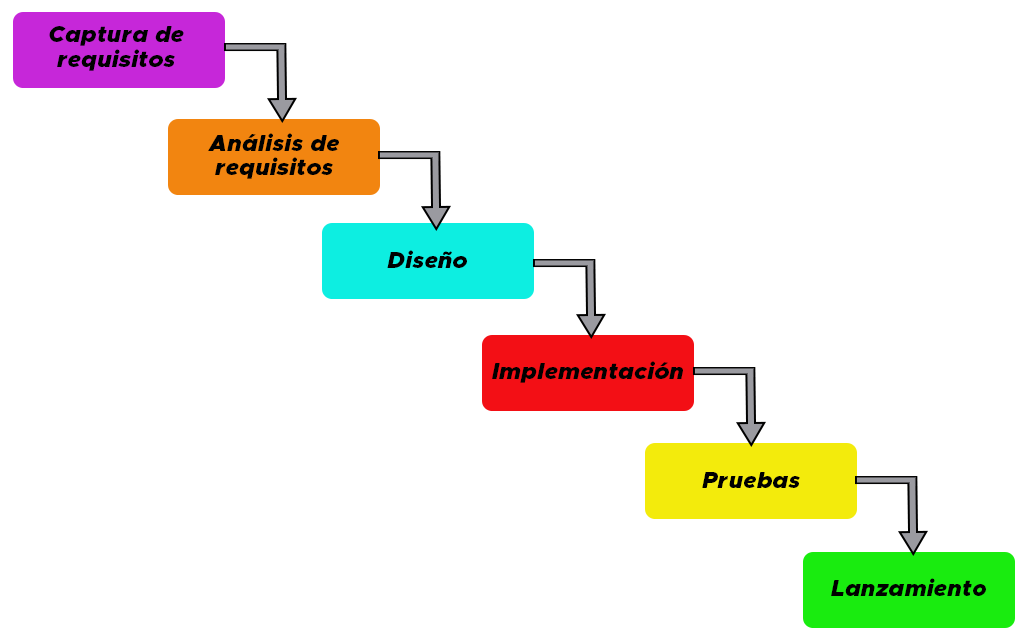
\includegraphics[width=1\textwidth]{Imagenes/Bitmap/etapasMetTradicional}\caption{Fases de una metodolog\'ia tradicional}
	%	\end{center}
	%\end{figure}
	\figura{Bitmap/etapasMetTradicional}{width=1\textwidth}{fig:etapasMetodologiaTradicional}{Fases de una metodolog\'ia tradicional}
	
	En cambio, en las metodolog\'ias \'agiles hay una lista de tareas, que se reparten entre los distintos grupos/subgrupos. \'estos suelen ser peque\~{n}os, de un tama\~{n}o m\'aximo de 10 personas. Cada tarea se trata de forma independiente, y son propensas a tener cambios (por ejemplo, es posible que una tarea inicial X, durante el desarrollo del proyecto, no se pueda realizar ya que no se ve viable), por lo que una tarea que estaba en una fase posterior s\'i puede volver a una fase previa. Todos estos cambios son los que hacen que genere valor para el cliente, por lo que la comunicaci\'on es fundamental en este tipo de metodolog\'ias.
	
	
	Hay diferentes metodolog\'ias \'agiles: \textit{XP}, \textit{Scrum}, \kanban, \textit{ScrumBan}, etc. Este proyecto seguir\'a la metodolog\'ia \kanban.


%------Segunda secci\'on: Kanban------%
\section{Kanban}
%-----------------------------------%
\label{cap3:sec:kanban}

	El t\'ermino ``\kanban``\space proviene del japon\'es, cuyo significado es ``tarjetas visuales``. Fue creado en la empresa Toyota para controlar el avance del trabajo con los materiales disponibles.
	
	Con \kanban \space puedes visualizar el trabajo hecho y por hacer, as\'i como las distintas fases por las que puede pasar una tarea, con el fin de que no se acumule el trabajo pendiente. Todo esto es posible ya que se utiliza una pizarra o tablero, ``tablero \kanban``\space (\textit{Kanban Board}). La calidad del trabajo y la productividad se ven aumentadas por la mejora del flujo de trabajo en equipo.
	
	Como uno de los objetivos de \kanban \space es saber el estado del proyecto en cada momento, y los grupos son reducidos, hay una limitaci\'on de tareas que podr\'a tener cada miembro del equipo en cada fase. Esto es el WIP (\textit{Work In Progress}).

\subsection{Tablero Kanban}
	
	Para representar las fases y las tareas se usa un tablero \kanban. Dicho tablero se divide en varias columnas que representan las distintas fases por las que puede pasar una tarea. Este tablero deber\'a tener, como m\'inimo, tres columnas:
	
	\begin{itemize}
		\item \textit{To Do}: En esta lista se tienen las tareas pendientes por realizar.
		\item \textit{Doing}: Cuando un grupo empieza a trabajar en una tarea, deber\'a moverla de ``\textit{To Do}`` a ``\textit{Doing}``.
		\item \textit{Done}: Tras saber que se ha realizado correctamente la tarea, y se ha dado por validada y aprobada, se podr\'a dar por terminada, por lo que se mover\'a a ``\textit{Done}``.
	\end{itemize}
	
	En la Figura \ref{fig:tableroKanban} se puede ver nuestro tablero \kanban \space en el inicio del proyecto. Las tres columnas que se requieren como m\'inimo est\'an presentes en nuestro tablero, pero, adem\'as, se han a\~{n}adido cuatro columnas extra:
	
	\begin{itemize}
		\item \textit{Backlog}: Corresponden con las tareas que no se pueden realizar en un presente, y que se podr\'an en un futuro.
		\item \textit{Document Review}: En esta columna se encuentran las tareas que requieren revisi\'on de memoria por parte del equipo. Estas tareas las revisar\'an quienes no hayan redactado el punto de memoria que dice la tarea.
		\item \textit{Needs Testing}: Al terminar de hacer una tarea de implementaci\'on, habr\'a que moverla de ``\textit{Doing}`` a ``\textit{Needs Testing}`` y habr\'a que pasarla en una serie de pruebas para comprobar que se ha realizado correctamente, y no da lugar a errores.
		\item \textit{Needs approval}: En esta lista se encuentran las tareas que necesitan ser aprobadas por las tutoras antes de darlas por finalizadas. Normalmente se encuentran las tareas que son de ``memoria``, aunque tambi\'en pueden aparecer de otro tipo.
	\end{itemize}
	
	\figura{Bitmap/tableroKanban}{width=1\textwidth}{fig:tableroKanban}{Tablero \kanban \space al inicio del proyecto}
	
	El WIP ser\'a de tres tareas en la columna ``\textit{In progress}``, y una en ``\textit{Needs testing}`` para cada miembro del equipo, ya que lo formamos tres personas. Hay varias excepciones en las que no se contempla el WIP, que son en ``\textit{Document Review}`` (cuando una persona realiza una tarea de redactar memoria, el resto deben revisarla en busca de incoherencias o errores en la redacci\'on, con lo cual puede haber tantas tareas de revisi\'on como de redacci\'on), y en ``\textit{Needs approval}`` (son tareas a la espera de aprobaci\'on o rechazo por parte de las tutoras).
	
	Algunas tareas podr\'an ser asignadas a varios usuarios en el caso de que sea extensa, o requiera que alguna o todas las partes necesiten hacer lo mismo. En la Figura \ref{fig:tareaVariosUsuarios}, se puede ver un ejemplo de este tipo de tarea, en el que todos los componentes del grupo han tenido que realizar un prototipo, por lo que solo se mover\'ia a ``\textit{Done}`` en el caso de que la lista est\'e completa.
	
	As\'i mismo, en la Figura \ref{fig:tableroKanban} se observa que las tareas tienen asignadas unas etiquetas de colores:
	
	\begin{itemize}
		\item \colorbox{naranja}{\textcolor{naranja}{123}} Tareas relacionadas con la memoria.
		\item \colorbox{rosa}{\textcolor{rosa}{123}} Corresponden con tareas de redacci\'on. Normalmente van en conjunto con las tareas de memoria.
		\item \colorbox{azul}{\textcolor{azul}{123}} En este color se encuentran las tareas que requieren una revisi\'on por parte del equipo. Normalmente van junto a las tareas de memoria.
		\item \colorbox{azulClaro}{\textcolor{azulClaro}{123}} Tareas que requieren un dise\~{n}o, ya sea un prototipo en papel, una interfaz de la aplicaci\'on, etc.
		\item \colorbox{rojo}{\textcolor{rojo}{123}} Tareas relacionadas con la implementaci\'on, es decir, el desarrollo de c\'odigo.
		\item \colorbox{morado}{\textcolor{morado}{123}} Aqu\'i se encuentran las tareas que requiere investigaci\'on, por parte del equipo, antes de empezar a codificar o realizar cualquier otro tipo de tarea.
		\item \colorbox{azulOscuro}{\textcolor{azulOscuro}{123}} Tareas que no corresponden con ninguna de las anteriores.
	\end{itemize}

	\figura{Bitmap/tareaVariosUsuarios}{width=1\textwidth}{fig:tareaVariosUsuarios}{Tarea asignada a varios usuarios}
	
%------\'ultima secci\'on: Tipos de pruebas------%
\section{Tipos de pruebas}
%--------------------------------------------%
\label{cap3:sec:pruebas}

	Debido a que vamos a usar componentes, es decir, ``piezas`` que son independientes entre s\'i, haremos pruebas unitarias.

\subsection{Pruebas unitarias}

	Una prueba unitaria se utiliza para comprobar que un m\'etodo implementado funciona como se esperaba. Debe cumplir una serie de caracter\'isticas:
	
	\begin{itemize}
		\item Deben ser \textbf{autom\'aticas}: se deben poder ejecutar sin que haya una intervenci\'on manual.
		\item Deben ser \textbf{completas}: es decir, deben cubrir la totalidad del c\'odigo.
		\item Deben ser \textbf{independientes}: debido a que se ha creado para comprobar una parte concreta del c\'odigo, no deber\'ia interferir con otras partes, y se deben poder ejecutar en cualquier entorno.
		\item Deben ser \textbf{repetibles}: se deben repetir todas las veces que queramos, y el resultado debe ser el mismo en todas.
	\end{itemize}

	Ventajas de las pruebas unitarias:
	
	\begin{itemize}
		\item \textbf{Aumento de la calidad} del c\'odigo: debido a que estas pruebas se ejecutan de forma regular, permite detectar errores a tiempo y poder corregirlos antes de completar el c\'odigo, y liberar la aplicaci\'on.
		\item \textbf{Facilitan los cambios}: se pueden aplicar cambios para mejorar el c\'odigo, ya que ese cambio solo afectar\'ia a una parte del c\'odigo. En el caso de que al aplicar el cambio \'este no estuviera correctamente realizado, es decir, no hiciera lo que esperase, la prueba unitaria nos avisar\'ia de que hay errores.
		\item \textbf{Reduce los tiempos} de integraci\'on: ya que podemos probar partes del c\'odigo sin disponer del c\'odigo completo.
		\item \textbf{Reduce el coste}: teniendo en cuenta que permite detectar errores tempranos, los tiempos de entrega mejoran respecto a no usarlos.
	\end{itemize}
	
	Para realizar las pruebas, hemos optado por usar \textit{Jest}\footnote{https://jestjs.io/es-ES/}, una librer\'ia de testing para \textit{Javascript}, que adem\'as es compatible con el \textit{framework} que hemos elegido (\textit{React}). \textit{Jest} tiene una instalaci\'on muy sencilla, de pocos pasos, y su configuraci\'on es m\'inima. La documentaci\'on es completa, y contiene lo necesario para poder desarrollar estos tipos de pruebas, junto con una serie de ejemplos, realizados paso a paso.
	
	Estas pruebas las desarrollar\'a y realizar\'a alguno de los miembros que no haya implementado esa parte del c\'odigo, y las har\'a cuando:
	
	\begin{enumerate}
		\item La persona que haya desarrollado el c\'odigo, haya completado dicha tarea.
		\item No tenga tareas pendientes en la columna ``\textit{Needs Testing}`` (el WIP en esa columna es de una tarea por persona).
	\end{enumerate}

	La raz\'on de esto es porque las personas que no han escrito el c\'odigo pueden sacar m\'as casos de prueba que las personas que lo han escrito.

% Variable local para emacs, para  que encuentre el fichero maestro de
% compilaci\'on y funcionen mejor algunas teclas r\'apidas de AucTeX
%%%
%%% Local Variables:
%%% mode: latex
%%% TeX-master: "../Tesis.tex"
%%% End:
%---------------------------------------------------------------------
%
%               Cap\'itulo 4 - Herramientas empleadas
%
%---------------------------------------------------------------------
\setlength{\parskip}{\baselineskip}

\chapter{Herramientas empleadas}

\begin{resumen}
	
	En este cap\'itulo se explican las herramientas y librer\'ias que se han empleado en la creaci\'on de los prototipos. En la secci\'on 4.1 se introduce la herramienta online Moqups. En la secci\'on 4.2 se ense\~{n}a el ``framework`` que se ha utilizado.
	
\end{resumen}
	
	Para realizar el prototipado, algunos hemos optado por hacerlo en papel, y otros en formato digital. Para formato digital, se han usado diferentes herramientas.
	
%------Primera secci\'on: Moqups------%
\section{Moqups}
%-----------------------------------%
\label{cap4:sec:moqups}

	Moqups\footnote{https://moqups.com/} es una p\'agina web enfocada en la creaci\'on de bocetos, prototipos, diagramas, etc. Es bastante completa: puedes dise\~{n}ar una interfaz, o simplemente ver c\'omo es el flujo de un algoritmo, arrastrando los distintos elementos (o plantillas) que podemos encontrar en una aplicaci\'on (barras de progreso, etiquetas o \textit{labels}, enlaces, diferentes tipos de ventanas, etc.) desde men\'u lateral al espacio de trabajo. 
	
	Existe la posibilidad de a\~{n}adir comentarios e iconos, y poder crear diferentes p\'aginas en un mismo proyecto (por ejemplo, crear varias vistas de una aplicaci\'on), as\'i como a\~{n}adir interacci\'on a los elementos (como por ejemplo, cuando le des clic a un bot\'on, \'este realice una funci\'on espec\'ifica). Tambi\'en es colaborativo, es decir, puedes invitar a m\'as miembros para trabajar en equipo; y permite la gesti\'on de roles.
	
	En la Figura \ref{fig:interfazMoqups} se puede ver la interfaz de un proyecto en blanco. Se observa que en el men\'u lateral de la izquierda, se encuentran los apartados para la creaci\'on del prototipo (plantillas, p\'aginas que tiene el proyecto, comentarios, im\'agenes, iconos, etc). En la parte superior de la p\'agina, se pueden crear figuras geom\'etricas y a\~{n}adir notas, as\'i como poder agregar a otros usuarios, y la posibilidad de exportar el proyecto como una serie de im\'agenes en formato PNG o PDF; y a formato HTML. Por \'ultimo, en el men\'u lateral de la derecha, podemos encontrar el formato de las diferentes p\'aginas (o componentes), y las interacciones disponibles (Figura \ref{fig:interaccionesMoqups}).
	
	\figura{Bitmap/interfazMoqups}{width=1\textwidth}{fig:interfazMoqups}{Interfaz de Moqups}
	
	\figura{Bitmap/interaccionesMoqups}{width=1\textwidth}{fig:interaccionesMoqups}{Men\'u lateral de interacciones}
	
	
%------Segunda secci\'on: React------%
\section{React}
%----------------------------------%
\label{cap4:sec:react}

	\textit{React}\footnote{https://es.reactjs.org/} es una librer\'ia de \textit{JavaScript}, creada por Facebook y de c\'odigo abierto, que permite crear interfaces de usuario interactivas de forma sencilla. Est\'a basada en la programaci\'on orientada a componentes, donde cada componente se puede ver como una funcionalidad distinta, es decir, como una ``pieza`` de un puzle.
	
	La ventaja de usar componentes es que, al ser independientes unos de otros, si en la carga de una p\'agina web falla uno en espec\'ifico, no afectar\'ia al resto de componentes, por lo que dicha p\'agina quedar\'ia cargada sin ese componente. As\'i mismo, al usar un DOM (Modelo de Objetos del Documento) virtual, deja que la propia librer\'ia actualice las partes que han cambiado, en lugar de actualizar todos los componentes.
	
	La sintaxis que emplea \textit{React} es muy parecida a la sintaxis HTML. Para definir los componentes, se emplean etiquetas definidas por el usuario dentro de c\'odigo \textit{Javascript}. Esta sintaxis se llama \textit{JSX}. No es obligatorio su uso, pero emple\'andolo facilita tanto la codificaci\'on como la lectura del c\'odigo. En la Figura \ref{fig:sinformatoJSX} se puede ver un ejemplo de una funcionalidad sin emplear el formato \textit{JSX}; y en la Figura \ref{fig:conformatoJSX}, la misma funcionalidad pero usando \textit{JSX}.
	
	\figura{Bitmap/reactSinJSX}{width=1\textwidth}{fig:sinformatoJSX}{Funcionalidad sin usar JSX}
	
	\figura{Bitmap/reactConJSX}{width=1\textwidth}{fig:conformatoJSX}{Funcionalidad empleando JSX}
	
	\textit{React} aporta rendimiento, flexibilidad y organizaci\'on de c\'odigo, frente a la creaci\'on de una p\'agina web de forma cl\'asica (es decir, sin usar ninguna librer\'ia o \textit{framework}).Tiene una documentaci\'on bastante completa, junto con un tutorial para aprender desde cero.
	

% Variable local para emacs, para  que encuentre el fichero maestro de
% compilaci\'on y funcionen mejor algunas teclas r\'apidas de AucTeX
%%%
%%% Local Variables:
%%% mode: latex
%%% TeX-master: "../Tesis.tex"
%%% End:
%\include{...}
%\include{...}
%\include{...}

% Ap\'endices
%\appendix
%%---------------------------------------------------------------------
%
%                          Parte 3
%
%---------------------------------------------------------------------
%
% Parte3.tex
% Copyright 2009 Marco Antonio Gomez-Martin, Pedro Pablo Gomez-Martin
%
% This file belongs to the TeXiS manual, a LaTeX template for writting
% Thesis and other documents. The complete last TeXiS package can
% be obtained from http://gaia.fdi.ucm.es/projects/texis/
%
% Although the TeXiS template itself is distributed under the 
% conditions of the LaTeX Project Public License
% (http://www.latex-project.org/lppl.txt), the manual content
% uses the CC-BY-SA license that stays that you are free:
%
%    - to share & to copy, distribute and transmit the work
%    - to remix and to adapt the work
%
% under the following conditions:
%
%    - Attribution: you must attribute the work in the manner
%      specified by the author or licensor (but not in any way that
%      suggests that they endorse you or your use of the work).
%    - Share Alike: if you alter, transform, or build upon this
%      work, you may distribute the resulting work only under the
%      same, similar or a compatible license.
%
% The complete license is available in
% http://creativecommons.org/licenses/by-sa/3.0/legalcode
%
%---------------------------------------------------------------------

% Definici�n de la �ltima parte del manual, los ap�ndices

\partTitle{Ap�ndices}

\makepart

%%---------------------------------------------------------------------
%
%                          Ap�ndice 1
%
%---------------------------------------------------------------------

\chapter{As� se hizo...}
\label{ap1:AsiSeHizo}

\begin{FraseCelebre}
\begin{Frase}
...
\end{Frase}
\begin{Fuente}
...
\end{Fuente}
\end{FraseCelebre}

\begin{resumen}
...
\end{resumen}

%-------------------------------------------------------------------
\section{Introducci�n}
%-------------------------------------------------------------------
\label{ap1:intro}

...

% Variable local para emacs, para  que encuentre el fichero maestro de
% compilaci�n y funcionen mejor algunas teclas r�pidas de AucTeX
%%%
%%% Local Variables:
%%% mode: latex
%%% TeX-master: "../Tesis.tex"
%%% End:

%\include{...}
%\include{...}
%\include{...}

\backmatter

%
% Bibliograf\'ia
%

%%---------------------------------------------------------------------
%
%                      configBibliografia.tex
%
%---------------------------------------------------------------------
%
% bibliografia.tex
% Copyright 2009 Marco Antonio Gomez-Martin, Pedro Pablo Gomez-Martin
%
% This file belongs to the TeXiS manual, a LaTeX template for writting
% Thesis and other documents. The complete last TeXiS package can
% be obtained from http://gaia.fdi.ucm.es/projects/texis/
%
% Although the TeXiS template itself is distributed under the 
% conditions of the LaTeX Project Public License
% (http://www.latex-project.org/lppl.txt), the manual content
% uses the CC-BY-SA license that stays that you are free:
%
%    - to share & to copy, distribute and transmit the work
%    - to remix and to adapt the work
%
% under the following conditions:
%
%    - Attribution: you must attribute the work in the manner
%      specified by the author or licensor (but not in any way that
%      suggests that they endorse you or your use of the work).
%    - Share Alike: if you alter, transform, or build upon this
%      work, you may distribute the resulting work only under the
%      same, similar or a compatible license.
%
% The complete license is available in
% http://creativecommons.org/licenses/by-sa/3.0/legalcode
%
%---------------------------------------------------------------------
%
% Fichero  que  configura  los  par�metros  de  la  generaci�n  de  la
% bibliograf�a.  Existen dos  par�metros configurables:  los ficheros
% .bib que se utilizan y la frase c�lebre que aparece justo antes de la
% primera referencia.
%
%---------------------------------------------------------------------


%%%%%%%%%%%%%%%%%%%%%%%%%%%%%%%%%%%%%%%%%%%%%%%%%%%%%%%%%%%%%%%%%%%%%%
% Definici�n de los ficheros .bib utilizados:
% \setBibFiles{<lista ficheros sin extension, separados por comas>}
% Nota:
% Es IMPORTANTE que los ficheros est�n en la misma l�nea que
% el comando \setBibFiles. Si se desea utilizar varias l�neas,
% terminarlas con una apertura de comentario.
%%%%%%%%%%%%%%%%%%%%%%%%%%%%%%%%%%%%%%%%%%%%%%%%%%%%%%%%%%%%%%%%%%%%%%
\setBibFiles{%
nuestros,latex,otros%
}

%%%%%%%%%%%%%%%%%%%%%%%%%%%%%%%%%%%%%%%%%%%%%%%%%%%%%%%%%%%%%%%%%%%%%%
% Definici�n de la frase c�lebre para el cap�tulo de la
% bibliograf�a. Dentro normalmente se querr� hacer uso del entorno
% \begin{FraseCelebre}, que contendr� a su vez otros dos entornos,
% un \begin{Frase} y un \begin{Fuente}.
%
% Nota:
% Si no se quiere cita, se puede eliminar su definici�n (en la
% macro setCitaBibliografia{} ).
%%%%%%%%%%%%%%%%%%%%%%%%%%%%%%%%%%%%%%%%%%%%%%%%%%%%%%%%%%%%%%%%%%%%%%
%\setCitaBibliografia{
%\begin{FraseCelebre}
%\begin{Frase}
%  Y as�, del mucho leer y del poco dormir, se le sec� el celebro de
%  manera que vino a perder el juicio.
%\end{Frase}
%\begin{Fuente}
%  Miguel de Cervantes Saavedra
%\end{Fuente}
%\end{FraseCelebre}
%}

%%
%% Creamos la bibliografia
%%
\makeBib

% Variable local para emacs, para  que encuentre el fichero maestro de
% compilaci�n y funcionen mejor algunas teclas r�pidas de AucTeX

%%%
%%% Local Variables:
%%% mode: latex
%%% TeX-master: "../Tesis.tex"
%%% End:


%
% \'indice de palabras
%

% S\'olo  la   generamos  si  est\'a   declarada  \generaindice.  Consulta
% TeXiS.sty para m\'as informaci\'on.

% En realidad, el soporte para la generaci\'on de \'indices de palabras
% en TeXiS no est\'a documentada en el manual, porque no ha sido usada
% "en producci\'on". Por tanto, el fichero que genera el \'indice
% *no* se incluye aqu\'i (est\'a comentado). Consulta la documentaci\'on
% en TeXiS_pream.tex para m\'as informaci\'on.
\ifx\generaindice\undefined
\else
%%---------------------------------------------------------------------
%
%                        TeXiS_indice.tex
%
%---------------------------------------------------------------------
%
% TeXiS_indice.tex
% Copyright 2009 Marco Antonio Gomez-Martin, Pedro Pablo Gomez-Martin
%
% This file belongs to TeXiS, a LaTeX template for writting
% Thesis and other documents. The complete last TeXiS package can
% be obtained from http://gaia.fdi.ucm.es/projects/texis/
%
% This work may be distributed and/or modified under the
% conditions of the LaTeX Project Public License, either version 1.3
% of this license or (at your option) any later version.
% The latest version of this license is in
%   http://www.latex-project.org/lppl.txt
% and version 1.3 or later is part of all distributions of LaTeX
% version 2005/12/01 or later.
%
% This work has the LPPL maintenance status `maintained'.
% 
% The Current Maintainers of this work are Marco Antonio Gomez-Martin
% and Pedro Pablo Gomez-Martin
%
%---------------------------------------------------------------------
%
% Contiene  los  comandos  para  generar  el �ndice  de  palabras  del
% documento.
%
%---------------------------------------------------------------------
%
% NOTA IMPORTANTE: el  soporte en TeXiS para el  �ndice de palabras es
% embrionario, y  de hecho  ni siquiera se  describe en el  manual. Se
% proporciona  una infraestructura  b�sica (sin  terminar)  para ello,
% pero  no ha  sido usada  "en producci�n".  De hecho,  a pesar  de la
% existencia de  este fichero, *no* se incluye  en Tesis.tex. Consulta
% la documentaci�n en TeXiS_pream.tex para m�s informaci�n.
%
%---------------------------------------------------------------------


% Si se  va a generar  la tabla de  contenidos (el �ndice  habitual) y
% tambi�n vamos a  generar el �ndice de palabras  (ambas decisiones se
% toman en  funci�n de  la definici�n  o no de  un par  de constantes,
% puedes consultar modo.tex para m�s informaci�n), entonces metemos en
% la tabla de contenidos una  entrada para marcar la p�gina donde est�
% el �ndice de palabras.

\ifx\generatoc\undefined
\else
   \addcontentsline{toc}{chapter}{\indexname}
\fi

% Generamos el �ndice
\printindex

% Variable local para emacs, para  que encuentre el fichero maestro de
% compilaci�n y funcionen mejor algunas teclas r�pidas de AucTeX

%%%
%%% Local Variables:
%%% mode: latex
%%% TeX-master: "./tesis.tex"
%%% End:

\fi

%
% Lista de acr\'onimos
%

% S\'olo  lo  generamos  si  est\'a declarada  \generaacronimos.  Consulta
% TeXiS.sty para m\'as informaci\'on.


\ifx\generaacronimos\undefined
\else
%---------------------------------------------------------------------
%
%                        TeXiS_acron.tex
%
%---------------------------------------------------------------------
%
% TeXiS_acron.tex
% Copyright 2009 Marco Antonio Gomez-Martin, Pedro Pablo Gomez-Martin
%
% This file belongs to TeXiS, a LaTeX template for writting
% Thesis and other documents. The complete last TeXiS package can
% be obtained from http://gaia.fdi.ucm.es/projects/texis/
%
% This work may be distributed and/or modified under the
% conditions of the LaTeX Project Public License, either version 1.3
% of this license or (at your option) any later version.
% The latest version of this license is in
%   http://www.latex-project.org/lppl.txt
% and version 1.3 or later is part of all distributions of LaTeX
% version 2005/12/01 or later.
%
% This work has the LPPL maintenance status `maintained'.
% 
% The Current Maintainers of this work are Marco Antonio Gomez-Martin
% and Pedro Pablo Gomez-Martin
%
%---------------------------------------------------------------------
%
% Contiene  los  comandos  para  generar  el listado de acr�nimos
% documento.
%
%---------------------------------------------------------------------
%
% NOTA IMPORTANTE:  para que la  generaci�n de acr�nimos  funcione, al
% menos  debe  existir  un  acr�nimo   en  el  documento.  Si  no,  la
% compilaci�n  del   fichero  LaTeX  falla  con   un  error  "extra�o"
% (indicando  que  quiz�  falte  un \item).   Consulta  el  comentario
% referente al paquete glosstex en TeXiS_pream.tex.
%
%---------------------------------------------------------------------


% Redefinimos a espa�ol  el t�tulo de la lista  de acr�nimos (Babel no
% lo hace por nosotros esta vez)

\def\listacronymname{Lista de acr�nimos}

% Para el glosario:
% \def\glosarryname{Glosario}

% Si se  va a generar  la tabla de  contenidos (el �ndice  habitual) y
% tambi�n vamos a  generar la lista de acr�nimos  (ambas decisiones se
% toman en  funci�n de  la definici�n  o no de  un par  de constantes,
% puedes consultar config.tex  para m�s informaci�n), entonces metemos
% en la  tabla de contenidos una  entrada para marcar  la p�gina donde
% est� el �ndice de palabras.

\ifx\generatoc\undefined
\else
   \addcontentsline{toc}{chapter}{\listacronymname}
\fi


% Generamos la lista de acr�nimos (en realidad el �ndice asociado a la
% lista "acr" de GlossTeX)

\printglosstex(acr)

% Variable local para emacs, para  que encuentre el fichero maestro de
% compilaci�n y funcionen mejor algunas teclas r�pidas de AucTeX

%%%
%%% Local Variables:
%%% mode: latex
%%% TeX-master: "../Tesis.tex"
%%% End:

\fi

%
% Final
%
%---------------------------------------------------------------------
%
%                      fin.tex
%
%---------------------------------------------------------------------
%
% fin.tex
% Copyright 2009 Marco Antonio Gomez-Martin, Pedro Pablo Gomez-Martin
%
% This file belongs to the TeXiS manual, a LaTeX template for writting
% Thesis and other documents. The complete last TeXiS package can
% be obtained from http://gaia.fdi.ucm.es/projects/texis/
%
% Although the TeXiS template itself is distributed under the 
% conditions of the LaTeX Project Public License
% (http://www.latex-project.org/lppl.txt), the manual content
% uses the CC-BY-SA license that stays that you are free:
%
%    - to share & to copy, distribute and transmit the work
%    - to remix and to adapt the work
%
% under the following conditions:
%
%    - Attribution: you must attribute the work in the manner
%      specified by the author or licensor (but not in any way that
%      suggests that they endorse you or your use of the work).
%    - Share Alike: if you alter, transform, or build upon this
%      work, you may distribute the resulting work only under the
%      same, similar or a compatible license.
%
% The complete license is available in
% http://creativecommons.org/licenses/by-sa/3.0/legalcode
%
%---------------------------------------------------------------------
%
% Contiene la �ltima p�gina
%
%---------------------------------------------------------------------


% Ponemos el marcador en el PDF al nivel adecuado, dependiendo
% de su hubo partes en el documento o no (si las hay, queremos
% que aparezca "al mismo nivel" que las partes.
\ifpdf
\ifx\tienePartesTeXiS\undefined
   \pdfbookmark[0]{Fin}{fin}
\else
   \pdfbookmark[-1]{Fin}{fin}
\fi
\fi

\thispagestyle{empty}\mbox{}

\vspace*{4cm}

\small

\hfill \emph{--�Qu� te parece desto, Sancho? -- Dijo Don Quijote --}

\hfill \emph{Bien podr�n los encantadores quitarme la ventura,}

\hfill \emph{pero el esfuerzo y el �nimo, ser� imposible.}

\hfill 

\hfill \emph{Segunda parte del Ingenioso Caballero} 

\hfill \emph{Don Quijote de la Mancha}

\hfill \emph{Miguel de Cervantes}

\vfill%space*{4cm}

\hfill \emph{--Buena est� -- dijo Sancho --; f�rmela vuestra merced.}

\hfill \emph{--No es menester firmarla -- dijo Don Quijote--,}

\hfill \emph{sino solamente poner mi r�brica.}

\hfill 

\hfill \emph{Primera parte del Ingenioso Caballero} 

\hfill \emph{Don Quijote de la Mancha}

\hfill \emph{Miguel de Cervantes}


\newpage
\thispagestyle{empty}\mbox{}

\newpage

% Variable local para emacs, para  que encuentre el fichero maestro de
% compilaci�n y funcionen mejor algunas teclas r�pidas de AucTeX

%%%
%%% Local Variables:
%%% mode: latex
%%% TeX-master: "../Tesis.tex"
%%% End:


\end{document}
